%% ESSD data description: per-cell record of directly measured seafloor in the GEBCO grid releases 2019-2026.
%% Build: docs/essd/build.sh (tectonic + bibtex with copernicus.bst).
%%
%% SOURCE CONVENTION. Every number in the text has a LaTeX comment (%% ...) naming the repository file and key it
%% comes from. Paths are relative to the repository root. "derived:" = simple arithmetic on the named file.
%%   G   = dataset/tables/global_by_release.csv
%%   RD  = dataset/tables/recoded_away_by_destination_tid.csv
%%   LB  = dataset/tables/by_latitude_band_by_release.csv
%%   DB  = dataset/tables/by_depth_bin_by_release.csv
%%   OC  = dataset/tables/by_ocean_by_release.csv
%%   ZN  = dataset/tables/by_zone_by_release.csv
%%   CS  = dataset/tables/cellsize_sensitivity_2026.csv ; SC = docs/sensitivity_cellsize.md
%%   VL  = dataset/build/verify.log ; CC = dataset/build/compliance_checker.txt ; DR = dataset/README.md
%%   H   = data/derived/history_stats.json ; S = data/derived/stats.json ; RG = data/derived/regions.json
%%   IC  = dataset/tables/inland_components.csv ; TC = dataset/tables/by_tid_code_by_release.csv
%%   VM  = data/derived/verify_mirror.json ; IN = dataset/inputs.sha256
%%   G23 = docs/gebco2023_tid_version.md ; DC = docs/data-contract.md
%% Derived numbers from the CSV files were recomputed on 2026-11-16 (script kept in the session scratchpad,
%% logic: sums of the *_km2 columns over the named rows).

\documentclass[essd, manuscript]{copernicus}

%% Dataset and code DOIs: not minted yet (see docs/essd/OPEN_ITEMS.md). Replace both lines once the deposits exist.
\newcommand{\datasetdoi}{10.5281/zenodo.24287579}
\newcommand{\codedoi}{10.5281/zenodo.24287662}

\newcommand{\as}{$^{\prime\prime}$}      % arc second
\newcommand{\am}{$^{\prime}$}            % arc minute
\newcommand{\kmsq}{km$^{2}$}
\newcommand{\Mkmsq}{M\,km$^{2}$}         % tables only

%% allow line breaks after underscores in long file and variable names
\let\usorig\_
\renewcommand{\_}{\usorig\allowbreak}
\emergencystretch=1.5em

\begin{document}

\title{A cell-level record of directly measured seafloor in the GEBCO grid releases 2019--2026}

\Author[1][ismoilovdev@gmail.com]{Otabek}{Ismoilov}

\affil[1]{Independent researcher, ORCID: \url{https://orcid.org/0009-0008-2785-3691}}

\runningtitle{Directly measured seafloor in GEBCO releases 2019--2026}

\runningauthor{O. Ismoilov}

\received{}
\pubdiscuss{}
\revised{}
\accepted{}
\published{}

\firstpage{1}

\maketitle

\begin{abstract}
Each annual General Bathymetric Chart of the Oceans (GEBCO) grid comes with a Type Identifier (TID) grid that codes, for every 15 arc-second cell, whether the depth was measured directly or estimated.
We present a cell-level record of directly measured seafloor built from the eight TID grids of GEBCO\_2019 to GEBCO\_2026.
For every cell of the global grid, an 8-bit mask states in which releases the cell is coded as directly measured (TID 10--17) inside one fixed ocean mask of 361.7 million km$^2$.
%% G ocean_area_km2 361,694,058
A per-cell flag marks the 0.93 million km$^2$ of the mask that lie below sea level but are not connected to the world ocean, mostly the Caspian Sea and the lowland around it.
%% G inland_below_sea_level_area_km2 931,885; IC rank 1 694,682
Derived variables and tidy tables summarise the record by release, latitude, depth, ocean, national waters, TID code and cell size, using exact spherical cell areas.
The measured share rises from 12.4\,\% in 2019 to 30.8\,\% in 2026.
%% G measured_share_fraction 2019 0.12427, 2026 0.30810
The coding is not cumulative: in each transition between releases, 0.8 to 4.6 million km$^2$ leave the measured codes, mostly to satellite-gravity prediction, interpolation or pre-generated grids.
%% G recoded_away_vs_previous_km2 min 764,863 (2025), max 4,624,417 (2020); RD
By 2026, 33.0\,\% of the seafloor has been coded as measured in at least one release.
%% G ever_measured_share_fraction 2026 0.33037
Because one sounding marks a whole cell, the share depends on cell size: 31.1\,\%, 33.5\,\% and 37.7\,\% on blocks about 463, 926 and 1853\,m wide.
%% CS ew1_any 0.31121, ew2_any 0.33518, ew4_any 0.37654
Statistics recomputed from the file match the reference values within 0.49\,km$^2$, all $3.7 \times 10^9$ cells match the eight source grids, and the global shares for 2019 and 2024 equal those of an earlier analysis to the precision given there (12.4\,\% and 28.5\,\%).
%% VL worst |diff| 0.490 km2; source GeoTIFF check, every cell: 3,732,480,000 cells, 0 mismatching; Niyazi et al. (2025) Results
The dataset is available under CC BY 4.0 at \url{https://doi.org/\datasetdoi} \citep{ismoilov2026data}.
\end{abstract}

\introduction

Most of the ocean floor is known only indirectly.
Global bathymetric grids fill the space between ship soundings with depths predicted from satellite-derived marine gravity \citep{smith1997,tozer2019}.
The Nippon Foundation--GEBCO Seabed 2030 Project aims to have the whole seafloor mapped by 2030 \citep{mayer2018,wolfl2019}.
With each annual GEBCO grid release it reports one number for progress: 15\,\% in 2019, rising to 28.7\,\% in 2026 \citep{news2019,news2026}.
%% G official_seabed2030_share_fraction 0.15 (2019), 0.287 (2026); quotes in pipeline/history.py OFFICIAL
The announcements give the percentage of the seafloor ``mapped'' (``mapped to modern standards'' in 2025 and 2026), but not a method by which it could be reproduced \citep{news2025,news2026}.
Seabed 2030 sets target grid resolutions of 100 to 800\,m that depend on depth \citep[Table~2]{mayer2018}, and \citet{niyazi2025} describe its criterion as at least one sounding per target cell.

Every GEBCO release since 2019 also includes a Type Identifier (TID) grid on the same 15\as\ grid as the depths \citep{gebcodoc2026}.
It codes the source of each cell: land; a direct measurement (codes 10--17: single beam, multibeam, seismic, isolated sounding, sounding from an electronic navigational chart, lidar, optical sensor, or a combination); an indirect estimate (codes 40--48, for example prediction from satellite gravity or interpolation); or an unknown source (codes 70--72).
GEBCO\_2014 already carried a similar source identifier grid \citep{weatherall2015}.
The TID grid is public and versioned, and it is the layer that users of GEBCO consult to decide whether a depth was measured.

\citet{niyazi2025} used the TID grids of 2019 to 2024 to compute the share of the seafloor coded as directly measured in each release (TID 1 to 17 in their definition; the codes in use are 10 to 17), with breakdowns by ocean, depth and exclusive economic zone (EEZ).
Their shares are totals per release.
To our knowledge, a per-cell record across releases has not been published.
Without it, one cannot ask when a cell was first coded as measured, whether it stays so in later releases, or what the share would be on a different cell size.

This paper describes such a record.
For each 15\as\ cell of the global grid, the dataset stores in which of the eight releases GEBCO\_2019 to GEBCO\_2026 the cell is coded as directly measured.
It adds derived per-cell variables and tidy tables of areas by release, latitude, depth, ocean, national waters and cell size.
Everything is computed from the public TID grids with one fixed ocean mask and exact spherical cell areas, and the code is open.
The dataset provides the per-release state of every cell and variables derived from it, a flag for the parts of the ocean mask that are not connected to the world ocean, tables of areas and shares (including the area that leaves the measured codes between releases, split by destination code, and the area of every TID code in every release), the share on blocks of other sizes for GEBCO\_2026, and a cell-by-cell comparison with the source grids.
The paper describes the files (Sect.~\ref{sec:files}), the inputs (Sect.~\ref{sec:inputs}), the methods (Sect.~\ref{sec:methods}), the validation (Sects.~\ref{sec:valmethods} and \ref{sec:valresults}), what the record contains (Sect.~\ref{sec:content}), the comparison with other estimates (Sect.~\ref{sec:comparison}) and the known issues (Sect.~\ref{sec:limits}).

\section{Data description}
\label{sec:files}

\subsection{Files and naming}

The dataset \citep{ismoilov2026data} consists of one netCDF file, ten comma-separated tables, a README with the data dictionary, two checksum files (\texttt{inputs.sha256}, \texttt{checksums.sha256}) and two verification reports (\texttt{verify.log}, \texttt{compliance\_checker.txt}).
The netCDF file \texttt{seafloor\_measured\_record\_2019\_2026.nc} holds the per-cell record (783\,337\,035 bytes; variables in Table~\ref{tab:variables}).
%% DR "Files" table; dataset/build/build_info.json bytes 783,337,035
It is netCDF-4 (HDF5) with CF-1.8 and ACDD-1.3 attributes, compressed with zlib level 4 and the shuffle filter, in chunks of $720 \times 1440$ cells (3$^\circ$ $\times$ 6$^\circ$).
%% DR "netCDF file"; pipeline/build_dataset.py CHUNK = (720, 1440)
The grid has $43\,200 \times 86\,400$ cells of 15\as\ (1/240$^\circ$), registered at cell centres, with latitude ascending from south to north and longitude from $-180$ to $180^\circ$.
%% DR "netCDF file"; pipeline/build_dataset.py H15, W15
This is the orientation and indexing of the GEBCO netCDF grids, so index $(i, j)$ in the record is index $(i, j)$ in \texttt{GEBCO\_<year>\_TID.nc}.
Cell centres are $\varphi_i = -90 + (i + 0.5)/240$ and $\lambda_j = -180 + (j + 0.5)/240$ in degrees, and cell edges are given as CF bounds.
The datum is WGS84.

\begin{table*}[t]
\caption{Variables of \texttt{seafloor\_measured\_record\_2019\_2026.nc}. All grid variables have dimensions (lat, lon) $= (43\,200, 86\,400)$. ``Outside the mask'' means outside the fixed ocean mask (Sect.~\ref{sec:mask}).}
\label{tab:variables}
\small
\begin{tabular}{p{0.25\textwidth}p{0.12\textwidth}p{0.55\textwidth}}
\tophline
Variable & Type & Content \\
\middlehline
\texttt{measured\_release\_flags} & int16 & Bitmask (int16: bit 7 does not fit a signed byte, and the CF-1.8 checker rejects unsigned types): bit $k$ (value $2^k$) set if the cell is directly measured in GEBCO\_$(2019+k)$, $k = 0, \dots, 7$; 0 outside the mask, no fill value. The full record; the other per-release variables are functions of it. \\
\texttt{first\_measured\_release} & int16 & First release in which the cell is measured (2019--2026); fill $-1$ if never measured or outside the mask. \\
\texttt{last\_measured\_release} & int16 & Last release in which the cell is measured; fill as above. \\
\texttt{n\_releases\_measured} & int8 & Number of releases in which the cell is measured (0--8); fill $-1$ outside the mask. \\
\texttt{measured\_in\_2026} & int8 & 1 if measured in GEBCO\_2026, else 0; fill $-1$ outside the mask. \\
\texttt{recoded\_away} & int8 & 1 if measured in at least one release 2019--2025 but not in GEBCO\_2026; fill $-1$ outside the mask. \\
\texttt{inland\_below\_sea\_level} & int8 & 1 if the cell is in the mask but not connected to the world ocean (Sect.~\ref{sec:inland}), else 0; fill $-1$ outside the mask. \\
\texttt{ocean\_mask} & int8 & 1 inside the fixed ocean mask, else 0. \\
\texttt{lat}, \texttt{lon}, \texttt{lat\_bnds}, \texttt{lon\_bnds} & float64 & Cell centres and edges (degrees north, degrees east). \\
\texttt{crs} & int32 & Grid mapping \texttt{latitude\_longitude}, WGS84. \\
\bottomhline
\end{tabular}
\end{table*}

Three relations hold in every cell: \texttt{n\_releases\_measured}~$>0$ if and only if \texttt{first\_measured\_release} is not the fill value; \texttt{recoded\_away}~$=1$ if and only if \texttt{n\_releases\_measured}~$>0$ and \texttt{measured\_in\_2026}~$=0$; and the last release is not earlier than the first.
A cell can be measured, re-coded and measured again.
The first, last and count variables therefore do not determine the state in each release; \texttt{measured\_release\_flags} does.
Global attributes give the title, summary, the GEBCO DOI of each release, the processing history (including the elevation source), the licence, the creator, and text definitions of ``measured'', the ocean mask, the area method, the GEBCO\_2023 TID version and the meaning of ``first measured''; \texttt{time\_coverage\_start} and \texttt{time\_coverage\_end} are the announcement dates of GEBCO\_2019 and GEBCO\_2026 (2019-06-13 and 2026-04-27).

Figure~\ref{fig:map} shows the first measured release aggregated to 4\am\ cells.
Cells first coded as measured in GEBCO\_2019 and GEBCO\_2020 cover most continental margins and the main transit lines.
Later releases add survey lines and blocks across the open ocean.

\begin{figure*}[t]
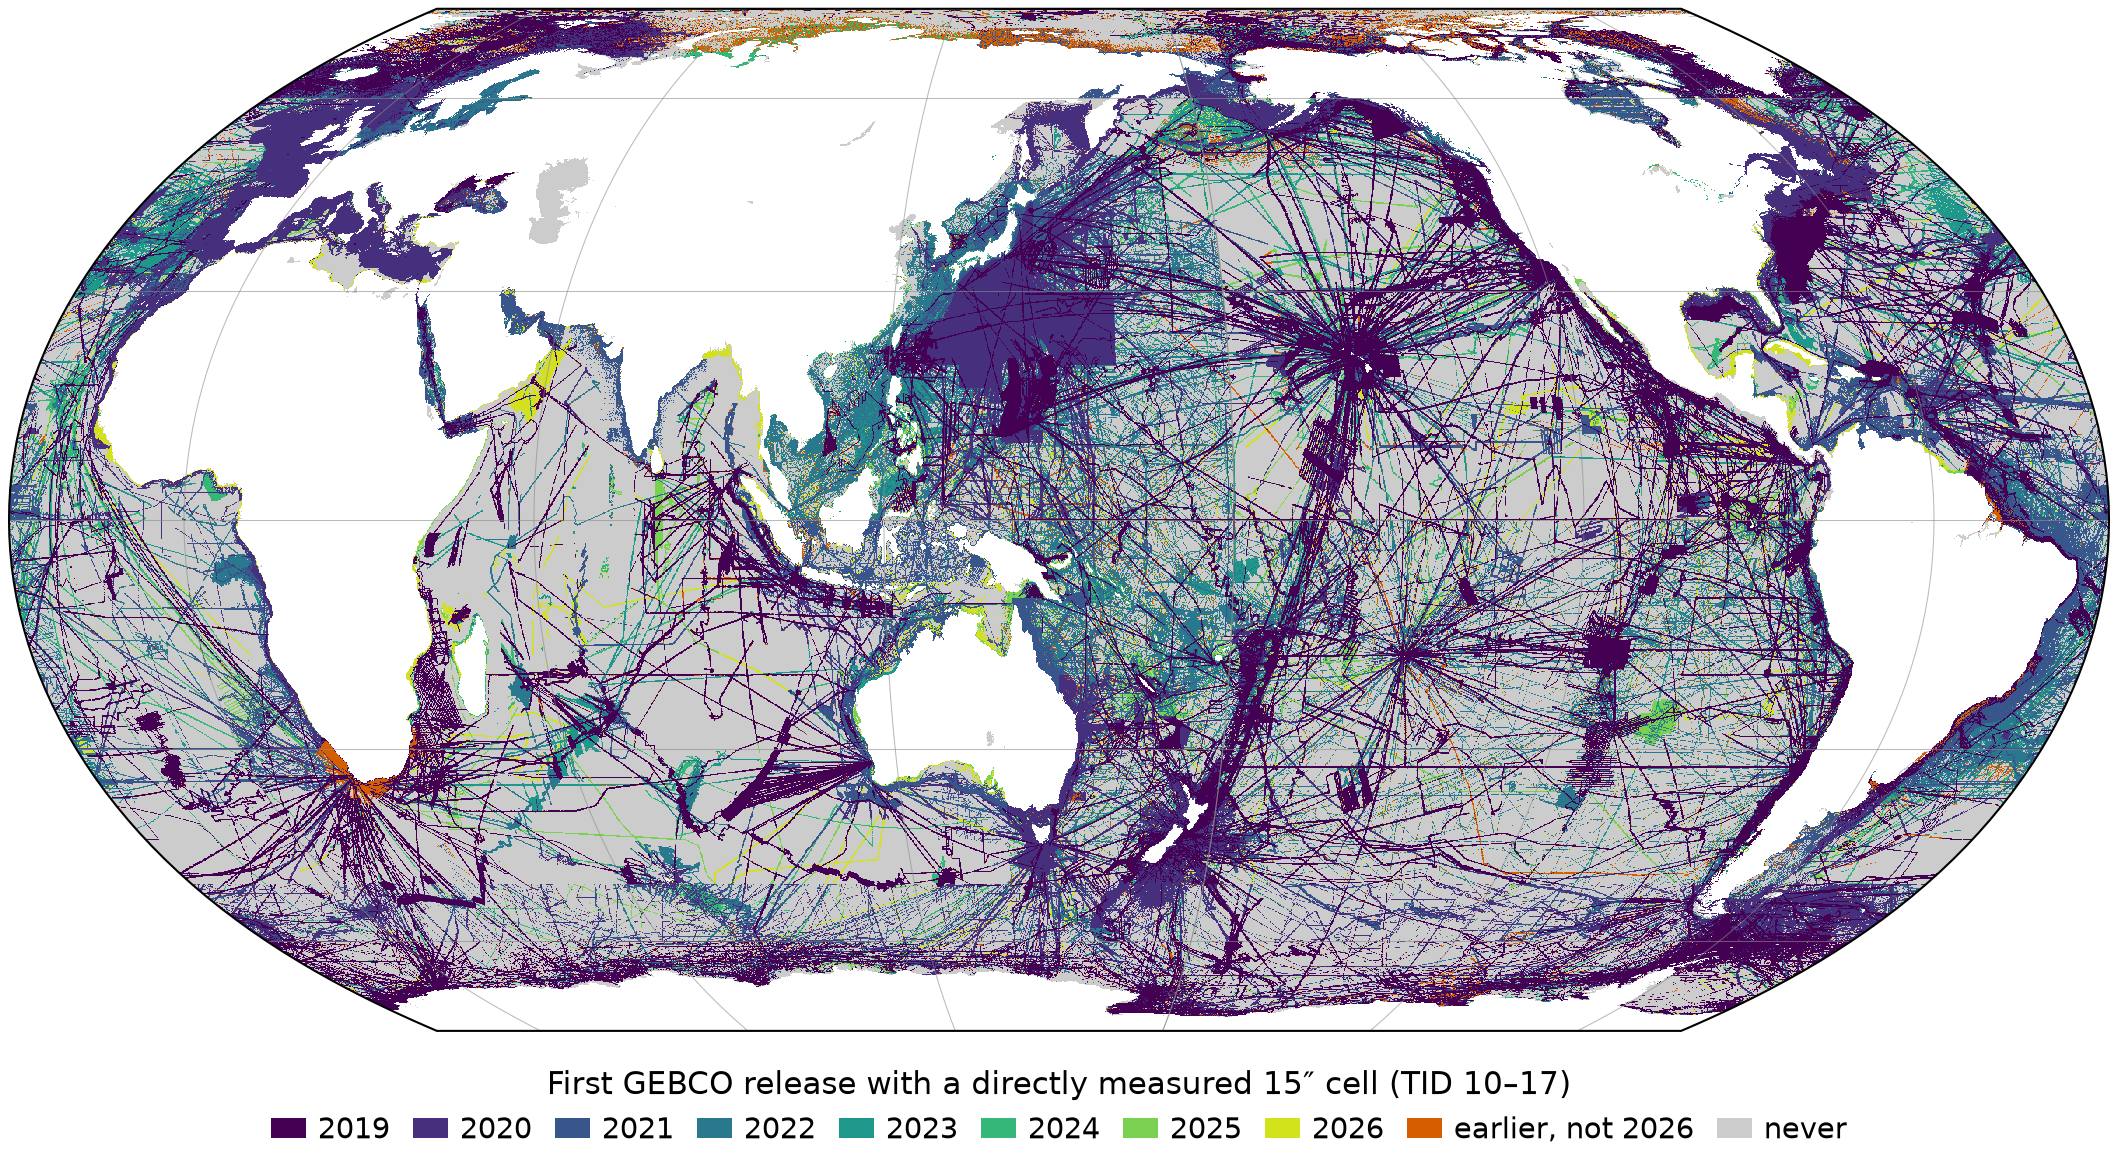
\includegraphics[width=\textwidth]{fig/fig01_first_measured_map.png}
\caption{First GEBCO release in which each part of the seafloor is coded as directly measured (TID 10--17), from the variable \texttt{measured\_release\_flags}. For display, the 15\as\ record was aggregated to 4\am\ cells ($16 \times 16$ cells): a 4\am\ cell takes the first release in which any of its 15\as\ cells is measured. This ``any'' rule widens single survey lines to at least one 4\am\ cell (about 7\,km at the equator), so lines look wider than they are. Vermillion (``earlier, not 2026'') marks 4\am\ cells in which at least one 15\as\ cell was measured in an earlier release and none is measured in GEBCO\_2026. Grey: ocean never coded as measured in 2019--2026. White: land and areas outside the fixed ocean mask, including the Antarctic ice sheet. The Caspian Sea and other areas flagged by \texttt{inland\_below\_sea\_level} are inside the mask (Sect.~\ref{sec:mask}). Equal Earth projection centred on 150$^\circ$\,E. Data: GEBCO Compilation Group, GEBCO\_2019 to GEBCO\_2026 TID grids.}
\label{fig:map}
\end{figure*}

\subsection{Tables}

The ten tables in \texttt{tables/} are UTF-8 comma-separated files with one header row, a full stop as decimal separator and no thousands separator.
%% DR "Tables"
Units are in the column names: \texttt{\_km2} for square kilometres (sums of exact 15\as\ cell areas, three decimals), \texttt{\_fraction} for dimensionless values between 0 and 1, \texttt{\_deg} for degrees and \texttt{\_m} for metres.
An empty field means ``not applicable'', for example the change relative to the previous release for 2019.
\begin{itemize}
\item \texttt{global\_by\_release.csv} (8 rows): per release, the ocean area, the measured area and share, the ever-measured area and share, the area first measured in that release, the area newly measured and re-coded away relative to the previous release, the share with each release's own mask, the official Seabed 2030 figure with its announcement date and source URL, and the area, measured area and measured share without the cells flagged \texttt{inland\_below\_sea\_level}.
\item \texttt{recoded\_away\_by\_destination\_tid.csv} (65 rows): for each transition, the area re-coded away split by the TID code the cells have in the later release.
\item \texttt{by\_latitude\_band\_by\_release.csv} (280 rows), \texttt{by\_depth\_bin\_by\_release.csv} (352 rows), \texttt{by\_ocean\_by\_release.csv} (96 rows) and \texttt{by\_zone\_by\_release.csv} (32 rows): the same quantities as the global table for 5$^\circ$ latitude bands, 250\,m depth bins, ocean basins and the split into EEZs and high seas, for every release. The Caspian Sea box (46--55.5$^\circ$\,E, 36--47.5$^\circ$\,N) is its own group in the ocean and zone tables and is included in the global figures.
\item \texttt{cellsize\_sensitivity\_2026.csv} (252 rows): the GEBCO\_2026 measured share on native cells and on six block variants, globally and per 5$^\circ$ band (Sect.~\ref{sec:cellsize}).
\item \texttt{by\_tid\_code\_by\_release.csv} (145 rows): the area of every TID code inside the mask, per release.
\item \texttt{inland\_components.csv} (186 rows): the components flagged \texttt{inland\_below\_sea\_level} of at least 100\,km$^2$, with bounding box, area and measured area in 2019 and 2026, and one row for all smaller ones (Sect.~\ref{sec:inland}).
\item \texttt{tid\_codes.csv} (21 rows): every TID code with its group (land, direct, indirect, unknown) and meaning.
\end{itemize}
%% DR "Files" table: row counts 8, 65, 280, 352, 96, 32, 252, 145, 186, 21 (wc -l minus header)
The file \texttt{inputs.sha256} gives the SHA-256 checksum of every input file (Sect.~\ref{sec:inputs}), and \texttt{checksums.sha256} that of the netCDF file, the tables, the README and \texttt{inputs.sha256}; the two reports are not checksummed because they are logs that change from run to run.
The README describes every column.

\subsection{Reading the record}

The state of a cell in release $Y$ is bit $Y - 2019$ of \texttt{measured\_release\_flags}.
An area-weighted share over any region is the sum of cell areas where that bit is set, divided by the sum of cell areas where \texttt{ocean\_mask} is 1.
Cell areas follow from \texttt{lat\_bnds} with Eq.~(\ref{eq:area}).
The dataset README gives a short Python example that computes the 2022 share for a box with xarray.
One full variable has $3.7 \times 10^9$ cells, so the file is best read in row strips or boxes aligned with the 720-row chunks.

\section{Input datasets}
\label{sec:inputs}

\subsection{GEBCO Type Identifier grids}

The record is built from the TID grids of the eight releases GEBCO\_2019 to GEBCO\_2026 \citep{gebco2019,gebco2020,gebco2021,gebco2022,gebco2023,gebco2024,gebco2025,gebco2026}.
Each is a global grid of $86\,400 \times 43\,200$ cells at 15\as.
%% pipeline/history.py H15, W15
The official netCDF archives were downloaded from the Centre for Environmental Data Analysis (CEDA) and converted to north-up GeoTIFF files with \texttt{gdal\_translate}, without resampling and with the codes stored as 8-bit integers.
%% DR "Provenance"; pipeline/history.py convert(); pipeline/fetch_data.sh (2026 TID from CEDA)
The orientation of every converted grid was checked against the netCDF metadata, and the record itself was compared with the converted grids cell by cell (Sect.~\ref{sec:valmethods}).

The GEBCO\_2023 TID grid exists in two issues with the same DOI and identical netCDF attributes.
GEBCO re-issued it in January 2024 to correct TID coding errors in the North Pacific and the central Mediterranean \citep{gebcodoc2026}.
%% G23 section 1: documentation in the CEDA zip, section 2.1
CEDA now serves only the re-issue, and this dataset uses it.
The two issues can be told apart only by checksum or by the file dates inside the archive (2023-04-24 for the original, 2024-02-12 for the re-issue).
%% G23 section 2 table: GEBCO_2023_TID.nc zip time
A cell-by-cell comparison shows 16\,542\,538 cells that differ, 2.80 million km$^2$ of them inside the ocean mask.
%% G23 section 3: 16,542,538 cells; 2,804,267 km2 in the mask
Most changes are in the Mediterranean (TID 41 to 17 or 70).
A further change on the Brazilian margin (24 to 18$^\circ$\,S), not mentioned in the GEBCO notes, moves 68\,479\,km$^2$ from code 17 to codes that are not direct.
%% G23 section 3 table: SW Atlantic off Brazil, -68,479 km2
With the original issue, the 2023 measured share would be 25.89\,\% instead of 26.27\,\%, and the area re-coded away in 2022--2023 would be 5.92 instead of 4.48 million km$^2$.
%% G23 section 4 table
The checksum of the converted file used here is in \texttt{inputs.sha256}.

\subsection{GEBCO\_2026 elevation}

The GEBCO\_2026 elevation (ice surface) was not read from CEDA but from a cloud-optimised GeoTIFF copy of the grid that the Australian Antarctic Division publishes on Source Cooperative \citep{aad2026gebcocog}: object \texttt{ausantarctic/gebco/GEBCO\_2026.tif} in the bucket \texttt{us-west-2.opendata.source.coop} (3\,286\,944\,666 bytes, last modified 7 May 2026).
According to its data-preparation notes, the copy was converted from the CEDA netCDF file with GDAL and its overviews were computed by average resampling.
The 1\am\ elevation behind the ocean mask and the depth bins is overview level 1 of that file, one value per $4 \times 4$ cells of 15\as, extracted with \texttt{gdal\_translate -ovr 1} (\texttt{pipeline/fetch\_data.sh}); the verification checks that it equals overview level 1 of a full local copy of the object in all 233\,280\,000 cells.
The full 15\as\ level is used only for the connectivity of the mask (Sect.~\ref{sec:inland}).
At six test sites ($16 \times 16$ cells each), the 15\as\ elevation of the copy was identical to the official CEDA grid read through OPeNDAP, and its 1\am\ values were within 0.82\,m of the mean of the $4 \times 4$ underlying 15\as\ cells (\texttt{pipeline/verify\_mirror.py}).
The SHA-256 checksums of both files are in \texttt{inputs.sha256}.
%% VM: 6 sites, elev_equal true at all; max ovr_max_abs_diff_vs_block_mean 0.8125 m; S3 listing 2026-11-16 (size, LastModified); VL "1' elevation vs overview level 1 ... 0 differing cells of 233,280,000"

\subsection{Regions}

Ocean basins come from Marine Regions' Global Oceans and Seas version 1 \citep{vliz2021goas}, EEZs from the Maritime Boundaries Geodatabase version 12 \citep{vliz2023eez} and the high seas from its High Seas layer version 2 \citep{vliz2024hs}.
All three are licensed CC BY 4.0.
EEZ boundaries include disputed areas and have no legal value.
The layers were not taken from the distributed shapefiles but from the Marine Regions GeoServer, as WMS GetMap responses in GeoJSON format in 72 tiles of 30$^\circ$ $\times$ 30$^\circ$ per layer requested at a pixel size of 1\am\ (\texttt{pipeline/regions.py}).
The server clips the polygons to each tile and generalises them at that pixel size; for the Belgian EEZ, 4136 vertices became 87, with a maximum shift of 0.43\am\ and an area change of $-0.24$\,\%.
%% docs/regions.md "Grid resolution" (spot check, Belgian EEZ)
The 216 tile files are not redistributed; their checksums are in \texttt{inputs.sha256}.

\subsection{Official figures}

For comparison, \texttt{global\_by\_release.csv} gives the share of the seafloor announced as mapped with each release: 15, 19, 20.6, 23.4, 24.9, 26.1, 27.3 and 28.7\,\% for 2019 to 2026 \citep{news2019,news2020,news2021,news2022,news2023,news2024,news2025,news2026}.
%% G official_seabed2030_share_fraction; each quote read on the cited page on 2026-11-15 (pipeline/history.py OFFICIAL)
Each value was read on the announcement page on 15 November 2026, and the URL is stored in the table.

\section{Methods}
\label{sec:methods}

\subsection{Ocean mask}
\label{sec:mask}

One mask is used for every release: GEBCO\_2026 TID not equal to 0 (land) and GEBCO\_2026 1\am\ elevation below 0, where the 1\am\ elevation is that of the 1\am\ cell containing the 15\as\ cell.
%% DR "Definitions"; pipeline/history.py
The elevation condition removes the Antarctic ice sheet, which the TID grid does not code as land.
Because the mask is fixed, differences between releases come from the TID codes alone.
The mask covers 361\,694\,058\,km$^2$.
%% G ocean_area_km2 361,694,058.130
Water under floating ice shelves is not part of the mask, because the grid holds the ice surface there.
The mask also keeps 931\,885\,km$^2$ below sea level that are not connected to the world ocean (Sect.~\ref{sec:inland}).
They are included in all published areas and shares, and flagged so that users can leave them out.
%% G inland_below_sea_level_area_km2 931,885.261

\subsection{Areas not connected to the world ocean}
\label{sec:inland}

The variable \texttt{inland\_below\_sea\_level} flags the cells of the mask that are not connected to the world ocean.
Connected components are computed on the 15\as\ grid with 8-connectivity, wrapping across 180$^\circ$, in strips of 720 rows whose labels are then merged across strip edges.
Connectivity is traced through the cells of the mask and through cells whose GEBCO\_2026 TID is not 0 and whose 15\as\ GEBCO\_2026 elevation is below 0.
The second set keeps straits narrower than a 1\am\ cell open (without it, the Bosporus closes and the Black Sea would be flagged); it does not add cells to the mask.
The component with the largest area is the world ocean; every other component of the mask is flagged.
%% pipeline/build_dataset.py connect_mask, merge_strips; tests/test_build_dataset.py (flood-fill reference with wrap)
The flagged area is 931\,885\,km$^2$ (0.26\,\% of the mask) in 8766 components.
%% G inland_below_sea_level_area_km2 931,885.261; VL "8766 components"; 931,885/361,694,058 = 0.258 %
It holds three kinds of area.
The first is basins below sea level away from the sea: the Caspian Sea together with the dry lowland of the Caspian Depression (694\,682\,km$^2$), the Qattara Depression (19\,395\,km$^2$), Lake Eyre (12\,837\,km$^2$), the Danakil Depression (7781\,km$^2$), Chott Melrhir (7464\,km$^2$), the Dead Sea with the Jordan Valley (4804\,km$^2$), the Salton Trough (4287\,km$^2$) and the Turpan Depression (3340\,km$^2$).
The second is lakes whose beds lie below 0\,m in the grid, for example Lake Superior (27\,086\,km$^2$ in its largest component), Lake Baikal (16\,680 and 5220\,km$^2$) and Lake Ontario (11\,813\,km$^2$).
The third is lagoons and inlets whose link to the sea the grid does not resolve, for example Lagoa Mirim (3746\,km$^2$) and the Curonian Lagoon (1502\,km$^2$).
%% IC ranks 1, 3, 5, 7, 8, 11, 12, 14 (basins); 2, 4, 9, 6 (lakes); 13, 19 (lagoons). Names from the bounding boxes.
Components of at least 100\,km$^2$ are listed with their bounding boxes in \texttt{inland\_components.csv}; the names there are given for orientation only.
Excluding the flagged cells changes the global measured share from 12.43 to 12.46\,\% in 2019 and from 30.81 to 30.89\,\% in 2026, because little of the flagged area is coded as measured (13\,718\,km$^2$ in 2026).
%% G measured_share_excluding_inland_fraction 2019 0.124591, 2026 0.308860; inland_below_sea_level_measured_area_km2 2026 13,718

\subsection{Directly measured}

A cell is measured in a release if its TID code in that release is 10--17 and it lies inside the mask.
All other codes inside the mask count as not measured.
A cell counts as measured whatever the number of soundings in it, so the share is a count of cells holding data, weighted by area.
A 15\as\ cell is 463\,m long in the north--south direction everywhere, but its east--west width shrinks with latitude: 463\,m at the equator, 232\,m at 60$^\circ$ and 80\,m at 80$^\circ$.
%% derived: 463.313 m * cos(phi)
Section~\ref{sec:cellsize} describes the variants that remove this effect.

\subsection{Cell areas}

Each 15\as\ cell is weighted by its exact area on a sphere of radius $R = 6371.0072$\,km, the authalic radius of the GRS80 ellipsoid \citep{moritz2000}.
For a cell between latitudes $\varphi_1 < \varphi_2$,
\begin{equation}
A = R^2\,\Delta\lambda\,(\sin\varphi_2 - \sin\varphi_1),
\label{eq:area}
\end{equation}
with $\Delta\lambda = 1/240^\circ$ in radians.
%% DR "Definitions"; pipeline/history.py row_area_km2, R_KM
The geodetic latitudes of the grid are used directly as latitudes on this sphere.
Compared with exact cell areas on the WGS84 ellipsoid, this makes the ocean area of a 5$^\circ$ band between 0.89\,\% too small (near the poles) and 0.45\,\% too large (near the Equator), and the whole mask 118\,801\,km$^2$ (0.033\,\%) too large.
The global measured share changes by at most 0.011 percentage points (2020) and by 0.002 points in 2026.
%% VL "sphere vs WGS84 ellipsoid": per band -0.886 % to +0.446 %; ocean mask 361,694,058 vs 361,575,258 km2; shares 2020 -0.0111, 2026 -0.0024 pp
All areas in the dataset are sums of 15\as\ cell areas, never cell counts.

\subsection{Per-cell record}

For each release $Y$, bit $Y - 2019$ of \texttt{measured\_release\_flags} is set where the cell is measured.
The other grid variables are computed from the bitmask: the first and last set bit, the number of set bits, bit 7 (GEBCO\_2026), and \texttt{recoded\_away} for cells with at least one set bit and bit 7 unset.
The grid is processed in strips of 720 rows by parallel worker processes; a full build takes a few minutes on a laptop.
%% pipeline/build_dataset.py STRIP = 720; dataset/build/build_info.json (4 workers)

\subsection{Summary tables}

For each release $Y$ and each group of cells, the tables give the measured area $m(Y)$, the area newly measured relative to $Y - 1$, the area measured in $Y - 1$ but not in $Y$ (``re-coded away''), the area measured in $Y$ or any earlier release (``ever measured'') and the area first measured in $Y$.
These satisfy
\begin{equation}
m(Y) = m(Y-1) + \mathrm{new}(Y) - \mathrm{recoded}(Y),
\label{eq:bookkeeping}
\end{equation}
and the first-measured areas summed over all releases equal the ever-measured area of 2026.
The area re-coded away is also split by the TID code the cells receive in the later release.
Latitude bands are 5$^\circ$ wide; a cell belongs to the band that contains its centre, and band edges fall on cell edges.
Depth bins are 250\,m wide and use the GEBCO\_2026 1\am\ depth for every release.
The Marine Regions polygons were rasterised onto the 1\am\ grid by cell centre, and each 15\as\ cell takes the region of its 1\am\ cell.
Overlapping claims and joint regimes are counted once in the EEZ total.
A ``neither'' zone holds ocean cells outside both polygon sets (areas below sea level away from the sea, and coastal slivers), and the Caspian Sea box is a separate zone that is included in the global figures.
%% DR "Tables"; ZN zones eez, high_seas, neither, caspian_sea_box

\subsection{Cell-size variants}
\label{sec:methods_cellsize}

To remove the east--west narrowing of 15\as\ cells, adjacent cells along a row at latitude $\varphi$ were merged into blocks of $k = \max(1, \mathrm{round}(1/\cos\varphi))$ cells, starting at 180$^\circ$\,W.
Blocks are then about 463\,m wide everywhere (309 to 618\,m, because $k$ is a whole number; $k = 1$ equatorward of 48.2$^\circ$).
%% SC "What was done"
To test block size itself, rows were also grouped into globally aligned sets of $s = 2$ or 4 rows with $k = \max(1, \mathrm{round}(s/\cos\varphi))$ columns, giving blocks of about 926 and 1853\,m in both directions.
%% SC; CS nominal_block_size_m 926.625, 1853.251
A block counts as measured if any of its ocean cells is measured (``any'' rule) or if more than half are (``majority'' rule).
The area of a block is the sum of the areas of its ocean cells, so the total ocean area is the same in every variant.
This analysis covers GEBCO\_2026 only (\texttt{pipeline/sensitivity\_cellsize.py}).

\subsection{Use of AI tools}
\label{sec:ai}

The code (the processing pipeline, the verification and the figure scripts), the analyses run with it, the figures, the dataset documentation and the first text of this manuscript were produced with the AI assistant Claude (Anthropic), used through Claude Code with the model claude-opus-5-5 (Claude Opus 5.5) as recorded in the session logs, between 13 and 16 November 2026, under the author's direction.
The author defined the questions and the scope, reviewed the outputs and takes responsibility for the content.
The AI assistant is not an author.

\section{Validation methods}
\label{sec:valmethods}

Eight checks test the dataset itself, and two comparisons relate it to other estimates.

\textit{Recomputation from the file.} A verification step (\texttt{pipeline/build\_dataset.py verify}) reads only the netCDF file.
It takes cell areas from \texttt{lat\_bnds} and \texttt{lon\_bnds} and recomputes, for each release, the measured, ever-measured and first-measured areas and shares and the areas newly measured and re-coded away.
The first-measured area is computed twice, from the bitmask and from \texttt{first\_measured\_release}.
The 2026 totals are recomputed from \texttt{n\_releases\_measured}, \texttt{measured\_in\_2026} and \texttt{recoded\_away}.
Each value is compared with the reference values that the history pipeline (\texttt{pipeline/history.py}), a separate code path with the same definitions, wrote before the record was built.
The tolerance is 1\,km$^2$ for areas (the reference stores whole square kilometres) and $10^{-9}$ for fractions.
%% DR "Verification"

\textit{Internal consistency.} The same step checks that every derived variable equals its function of the bitmask in every cell, that no bit is set outside the ocean mask, and that the cell areas add up to the area of the sphere.

\textit{Agreement with the source grids.} Global sums cannot detect a north--south flip of the grid.
The bitmask and the ocean mask were therefore compared, in every cell, with values recomputed from the eight source TID grids and the 1\am\ elevation, reading the file in strips of 720 rows located through the netCDF latitude coordinate.
The same step checks that the 1\am\ elevation file equals overview level 1 of the 15\as\ mirror file in every cell, that \texttt{inland\_below\_sea\_level} is 0 or 1 inside the mask and the fill value outside it, and that its area equals that of the connectivity step.

\textit{Separate code paths.} The GEBCO\_2026 measured share was also computed by three scripts that use the same definitions but separate code and different aggregation: on 15\as\ cells weighted by the cosine of the row latitude (\texttt{coverage.py}), on 15\as\ cells with exact areas (\texttt{history.py}), and on 1\am\ cells holding a measured fraction stored in steps of 1/254 (\texttt{regions.py}); all three are in \texttt{pipeline/}. These are not independent validations.

\textit{Bookkeeping.} Equation~(\ref{eq:bookkeeping}) was evaluated for every pair of consecutive releases, globally and in each table.

\textit{Mask choice.} The measured share was also computed with each release's own mask (its own TID not equal to 0, with the same elevation condition).

\textit{Area model.} The spherical cell areas were compared with exact cell areas on the WGS84 ellipsoid for the ocean area and the measured share of every release (Sect.~\ref{sec:methods}).

\textit{Conventions.} The file was tested with the IOOS compliance checker version 6.1.0 against CF-1.8 and ACDD-1.3.

\textit{Comparison with \citet{niyazi2025}.} The shares stated in their text (global for 2019 and 2024; by basin, depth zone and EEZ, mostly for 2024) are compared with the same groups in the tables of this dataset (Sect.~\ref{sec:comparison}).

\textit{Comparison with the official figures.} The official share for each release is compared with the measured share of the record (Sect.~\ref{sec:comparison}).
Because the two definitions differ, this is a comparison, not a validation.

\section{Validation results}
\label{sec:valresults}

Table~\ref{tab:validation} summarises the results.
All 67 quantities recomputed from the netCDF file agree with the reference values.
%% VL: 67 lines ending in OK
The largest difference is 0.49\,km$^2$ for areas and $4.1 \times 10^{-15}$ for fractions.
%% VL worst |diff| 0.490 km2, 4.1e-15
No cell has a derived variable that disagrees with the bitmask, and no bit is set outside the ocean mask.
All 3\,732\,480\,000 cells, holding 4\,706\,861\,838 measured bits, match the values recomputed from the source grids, and the 1\am\ elevation equals overview level 1 of the 15\as\ copy in all 233\,280\,000 cells.
%% VL "source GeoTIFF check, every cell: 3,732,480,000 cells, 4,706,861,838 measured bits, 0 mismatching cells"; "0 differing cells of 233,280,000"
The flag \texttt{inland\_below\_sea\_level} takes only valid values, and its area equals that of the connectivity step (931\,885\,km$^2$).
%% VL "inland_below_sea_level: cells with invalid value or fill not matching the mask: 0; area 931,885.261 km2 (connectivity pass 931,885.261 km2"

The three scripts give a GEBCO\_2026 share of 30.810\,\%, 30.810\,\% and 30.809\,\%.
%% S measured_fraction_area 0.3081019; H years[7].measured_frac 0.3081019; RG global_check measured_fraction 0.3080868
The 1\am\ variant differs in the third decimal because its stored fraction is quantised and because its ocean area is 361\,896\,286\,km$^2$ rather than 361\,694\,058\,km$^2$ (it counts the full area of every 1\am\ cell that contains at least one cell of the mask).
%% RG global_check ocean_area_km2 361,896,286.6 ; G ocean_area_km2 361,694,058.1
The bookkeeping identity holds to 0.001\,km$^2$ in the published tables, which is the rounding of the three-decimal values.
%% derived from G: max |m(Y) - m(Y-1) - new + recoded| = 0.001 km2
The reference pipeline asserts the same identity to 5\,km$^2$ on whole-kilometre values.
%% DC "Numbers": bookkeeping holds to < 5 km2 every year
With each release's own mask, the share changes by at most 0.016 percentage points (2023).
%% derived from G: max (measured_share_own_mask_fraction - measured_share_fraction) = 0.000158 (2023)

The compliance checker reports that all CF-1.8 tests pass.
%% CC "cf:1.8 ... All tests passed!"
For ACDD-1.3, no required attribute is missing.
It lists a missing \texttt{standard\_name} for \texttt{n\_releases\_measured}, for which no CF standard name exists, recommended attributes that are not set (\texttt{creator\_email}, \texttt{publisher\_*}, the vertical extent and the time resolution), the absence of a time variable against which \texttt{time\_coverage\_start} and \texttt{time\_coverage\_end} could be tested, and a mismatch between the geospatial bounds ($\pm 90^\circ$, $\pm 180^\circ$) and the outermost cell centres.
%% CC acdd:1.3 section
The bounds are deliberately the cell edges, consistent with \texttt{geospatial\_bounds}.
A second checker, \texttt{cfchecks}, could not be run because the UDUNITS-2 library it needs was not installed on the build computer.
%% DR "Conventions check"

\begin{table}[t]
\caption{Technical validation of the dataset. ``Reference'' values are those of the history pipeline, a separate code path with the same definitions (\texttt{data/derived/history\_stats.json}).}
\label{tab:validation}
\small
\begin{tabular}{p{0.42\textwidth}p{0.5\textwidth}}
\tophline
Check & Result \\
\middlehline
Recompute 67 area and share values from the netCDF file & All within tolerance; worst 0.49\,km$^2$ and $4.1 \times 10^{-15}$ \\
Derived variables vs bitmask, every cell & 0 disagreeing cells \\
Bits set outside the ocean mask & 0 \\
Bitmask and mask vs source grids, every cell & 3\,732\,480\,000 cells, 0 mismatches \\
1\am\ elevation vs overview level 1 of the 15\as\ copy & 233\,280\,000 cells, 0 differences \\
\texttt{inland\_below\_sea\_level}: values, area & 0 invalid cells; area equals the connectivity step \\
GEBCO\_2026 share by three scripts & 30.810, 30.810 and 30.809\,\% \\
Bookkeeping, Eq.~(\ref{eq:bookkeeping}), all transitions & Closes to 0.001\,km$^2$ (tables), $< 5$\,km$^2$ (reference) \\
Fixed vs each release's own mask & At most 0.016 percentage points \\
Sphere vs WGS84 ellipsoid & Ocean area $+0.033$\,\%; share at most 0.011 points \\
CF-1.8 (IOOS compliance checker 6.1.0) & All tests passed \\
Global share vs \citet{niyazi2025}, 2019 and 2024 & 12.43 vs 12.4\,\%; 28.54 vs 28.5\,\% (other groups: Table~\ref{tab:niyazi}) \\
\bottomhline
\end{tabular}
%% rows: VL; VL; VL; VL; VL; VL; S/H/RG; G and DC; G; VL; CC; G + Niyazi et al. 2025 Results
\end{table}

\section{Content of the record}
\label{sec:content}

This section describes what the record contains, with the numbers that a user is most likely to need.
The full set is in the tables.

\subsection{Measured share per release}

The area coded as directly measured grows from 44.9 million km$^2$ in GEBCO\_2019 to 111.4 million km$^2$ in GEBCO\_2026, or from 12.4\,\% to 30.8\,\% of the ocean (Table~\ref{tab:global}, Fig.~\ref{fig:share}).
%% G measured_area_km2 44,947,953 and 111,438,640; measured_share_fraction 0.12427, 0.30810
The largest newly coded area is in the transition from 2019 to 2020, 25.7 million km$^2$.
%% G new_vs_previous_km2 2020 25,654,489
The smallest newly coded area is in 2025 (4.9 million km$^2$).
%% G new_vs_previous_km2 2025 4,917,578
In the 0--250\,m depth bin, the measured share was 1.6\,\% in 2019 and 30.9\,\% in 2026.
%% derived from DB: bin 0-250 m, 2019 0.0160, 2026 0.3091
In the 2020 release alone, 4.4 million km$^2$ of this bin, 16\,\% of its area, was newly coded as measured.
%% DB 0-250 m 2020 new_vs_previous_km2 4,419,708; ocean_area_km2 27,926,268; ratio 0.158

\begin{table*}[t]
\caption{Directly measured share of the seafloor in each GEBCO release (TID 10--17, fixed ocean mask of 361.7\,\Mkmsq, exact spherical areas), the share measured in this or any earlier release, the changes relative to the previous release, and the official Seabed 2030 figure. Source: \texttt{global\_by\_release.csv}.}
\label{tab:global}
\begin{tabular}{lrrrrrrr}
\tophline
Release & Measured & Measured & Ever & New & Re-coded & Official & Difference \\
 & (\Mkmsq) & (\%) & measured (\%) & (\Mkmsq) & away (\Mkmsq) & (\%) & (pp) \\
\middlehline
2019 & 44.95 & 12.43 & 12.43 & -- & -- & 15.0 & $-2.57$ \\
2020 & 65.98 & 18.24 & 19.52 & 25.65 & 4.62 & 19.0 & $-0.76$ \\
2021 & 79.26 & 21.91 & 23.49 & 17.35 & 4.06 & 20.6 & $+1.31$ \\
2022 & 91.67 & 25.35 & 26.82 & 14.48 & 2.07 & 23.4 & $+1.95$ \\
2023 & 95.02 & 26.27 & 28.70 & 7.83 & 4.48 & 24.9 & $+1.37$ \\
2024 & 103.23 & 28.54 & 30.39 & 10.00 & 1.80 & 26.1 & $+2.44$ \\
2025 & 107.38 & 29.69 & 31.47 & 4.92 & 0.76 & 27.3 & $+2.39$ \\
2026 & 111.44 & 30.81 & 33.04 & 6.57 & 2.51 & 28.7 & $+2.11$ \\
\bottomhline
\end{tabular}
%% G all columns; Difference = 100*measured_share_fraction - 100*official_seabed2030_share_fraction
\belowtable{pp: percentage points (this record minus the official figure).}
\end{table*}

\begin{figure}[t]
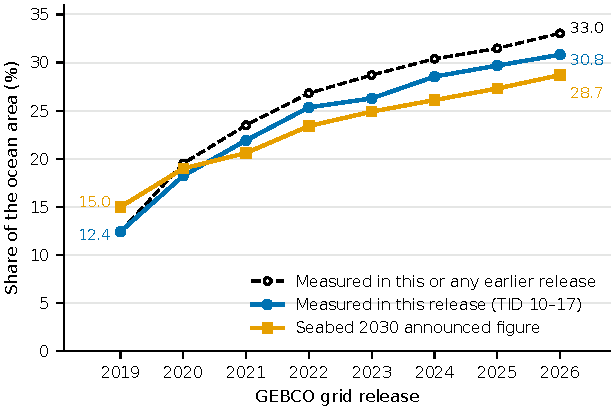
\includegraphics[width=12cm]{fig/fig02_share_by_release.pdf}
\caption{Share of the ocean area coded as directly measured (TID 10--17) in each GEBCO release, the share coded as measured in this or any earlier release, and the share announced by Seabed 2030 with each release. Fixed ocean mask of 361.7 million km$^2$. Data: \texttt{global\_by\_release.csv}; official figures from the release announcements \citep{news2019,news2020,news2021,news2022,news2023,news2024,news2025,news2026}.}
\label{fig:share}
\end{figure}

\subsection{Re-coding between releases}

The measured area does not only grow.
In every transition, part of the area coded as measured in one release is coded as not measured in the next: 4.62 million km$^2$ in 2020, 4.06 in 2021, 2.07 in 2022, 4.48 in 2023, 1.80 in 2024, 0.76 in 2025 and 2.51 in 2026 (Table~\ref{tab:global}, Fig.~\ref{fig:recoded}).
%% G recoded_away_vs_previous_km2
Over the seven transitions, 86.8 million km$^2$ entered the measured codes and 20.3 million km$^2$ left them.
%% derived from G: sum new_vs_previous_km2 86,794,561; sum recoded_away_vs_previous_km2 20,303,873; 44,947,953 + 86,794,561 - 20,303,873 = 111,438,640
Summed over all transitions, 48.5\,\% of the re-coded area moved to TID 40 (prediction from satellite gravity), 18.5\,\% to TID 70 (pre-generated grid), 18.0\,\% to TID 41 (interpolation) and 14.1\,\% to TID 44 (multiple sources in a gridded data set guided by satellite gravity).
%% derived from RD: area_km2 summed over transitions per destination_tid / 20,303,873
Less than 1\,\% went to other codes, including land.
%% derived from RD: codes 0, 42, 43, 45, 47, 48, 71, 72 together 0.9 %
The mix differs between transitions: in 2020, 56.7\,\% of the re-coded area went to TID 40, and in 2021, 37.7\,\% went to TID 70.
%% RD 2019->2020 TID 40 share_of_transition_fraction 0.567; 2020->2021 TID 70 0.377

\begin{figure}[t]
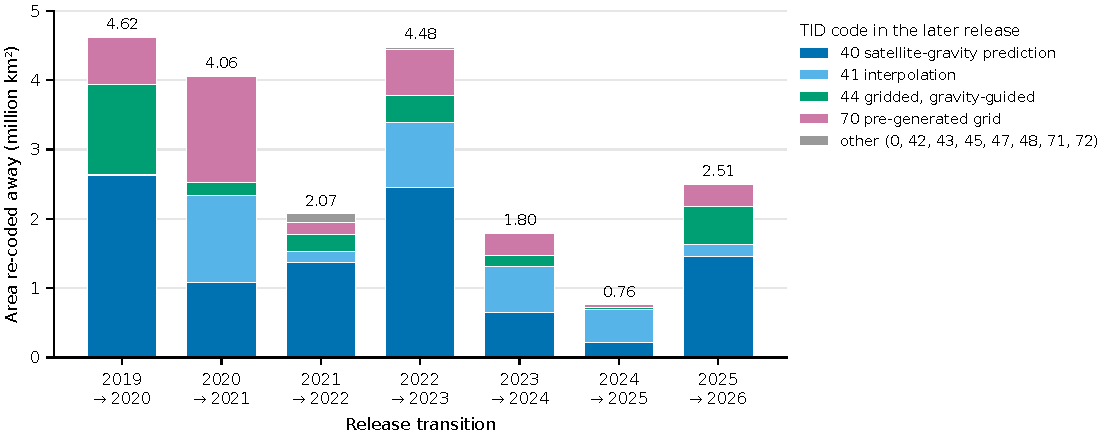
\includegraphics[width=\textwidth]{fig/fig03_recoded_by_destination.pdf}
\caption{Area coded as directly measured in one GEBCO release and not in the next (``re-coded away''), split by the TID code it has in the later release. Numbers above the bars are the totals in million km$^2$. ``Other'' groups codes 0 (land inside the fixed ocean mask), 42, 43, 45, 47, 48, 71 and 72, which together hold 0.9\,\% of the re-coded area. Data: \texttt{recoded\_away\_by\_destination\_tid.csv}.}
\label{fig:recoded}
\end{figure}

Some re-coded cells are coded as measured again in a later release.
By 2026, 119.5 million km$^2$ (33.0\,\%) have been coded as measured in at least one release, against 111.4 million km$^2$ (30.8\,\%) in GEBCO\_2026.
%% G 2026 ever_measured_area_km2 119,492,714, ever_measured_share_fraction 0.33037
The difference, 8.05 million km$^2$, is the area flagged by \texttt{recoded\_away}; it is 2.2\,\% of the ocean and 6.7\,\% of the ever-measured area.
%% G 2026 measured_earlier_not_in_this_release_km2 8,054,074; /361,694,058 = 0.0223; /119,492,714 = 0.0674
The ever-measured share is an upper bound: it also keeps cells that GEBCO later re-coded because an earlier code was wrong, as for the GEBCO\_2023 issue described in Sect.~\ref{sec:inputs}.

The flagged area is not spread evenly with latitude.
North of 65$^\circ$\,N, which holds 3.8\,\% of the ocean area, 15.7\,\% of the ever-measured area is not coded as measured in 2026; south of 60$^\circ$\,S the value is 9.4\,\%, against 6.7\,\% globally.
%% derived from LB 2026, bands lat_south_deg >= 65: ocean 13,707,475 km2 (3.8 %); (ever - measured)/ever = 0.157; bands lat_north_deg <= -60: 0.094; global 0.067
The record does not attribute a re-coding to a cause.

\subsection{Dependence on cell size}
\label{sec:cellsize}

On blocks about 463\,m wide at every latitude, the GEBCO\_2026 measured share is 31.12\,\% with the any rule and 30.60\,\% with the majority rule, against 30.81\,\% on native cells (Fig.~\ref{fig:cellsize}).
%% CS global: native 0.30810, ew1_any 0.31121, ew1_majority 0.30602
All of the increase under the any rule comes from rows poleward of 48.2$^\circ$, where cells are merged.
%% SC "Interpretation": all of the +0.31 points from rows poleward of 48.2 deg
The high-latitude bands rise by at most 5.7 percentage points (65--70$^\circ$\,N, from 38.66 to 44.32\,\%), and at 80--85$^\circ$\,N by 1.3 points (17.5 to 18.8\,\%).
%% CS bands: 65-70 N native 0.3866, ew1_any 0.443; 80-85 N 0.1751, 0.188 (SC table)
On these blocks, the bands north of 80$^\circ$\,N remain below the global share.

Block size has a larger effect than latitude.
With the any rule, the global share rises to 33.52\,\% on blocks of about 926\,m and to 37.65\,\% on blocks of about 1853\,m.
With the majority rule it stays between 29.98 and 30.60\,\%.
%% CS global: ew2_any 0.33518, ew4_any 0.37654; ew2_majority 0.29982, ew1_majority 0.30602, ew4_majority 0.30206
A share defined as ``one sounding per cell'' thus grows with the cell size, by 6.8 percentage points between the native grid and blocks of about 1.85\,km.
%% derived from CS: 37.654 - 30.810 = 6.84
A coverage figure therefore needs the cell size and the counting rule with which it was computed.

\begin{figure*}[t]
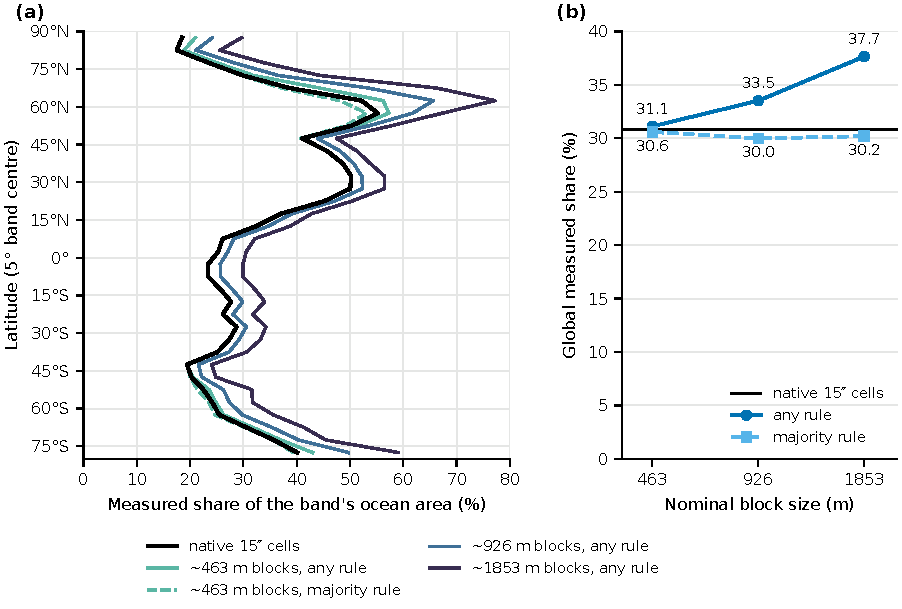
\includegraphics[width=\textwidth]{fig/fig04_cellsize_latitude.pdf}
\caption{Measured share of GEBCO\_2026 on native 15\as\ cells and on blocks of near-constant width. (a) Share per 5$^\circ$ latitude band, plotted at the band centre; the majority-rule variants at about 926 and 1853\,m lie close to the native curve and are omitted for clarity (all values are in the table). The band 80--85$^\circ$\,S, which holds 32\,km$^2$ of ocean, is not shown. (b) Global share against nominal block size for the any rule (a block counts as measured if any of its ocean cells is) and the majority rule (if more than half are). Data: \texttt{cellsize\_sensitivity\_2026.csv}.}
\label{fig:cellsize}
\end{figure*}

\subsection{Depth, latitude and jurisdiction}

The abyssal seafloor at 3--6\,km makes up 74.4\,\% of the ocean area and is 28.1\,\% measured in GEBCO\_2026, against 12.8\,\% in GEBCO\_2019 (Fig.~\ref{fig:depth}).
%% derived from DB: bins 3000-6000 m, area 0.744 of total; measured share 2026 0.281, 2019 0.128
The 4--5\,km range alone holds 31.9\,\% of the ocean area and has the lowest share of any 1\,km range, 26.7\,\%.
%% derived from DB 2026: 4000-5000 m area 0.319, share 0.267
Depths of 1--3\,km are 41.6\,\% measured.
%% derived from DB 2026: 1000-3000 m share 0.416
Depths greater than 7\,km cover 0.1\,\% of the area and are 93.6\,\% measured.
%% derived from DB 2026: 7000-11000 m area 0.0011, share 0.936

\begin{figure}[t]
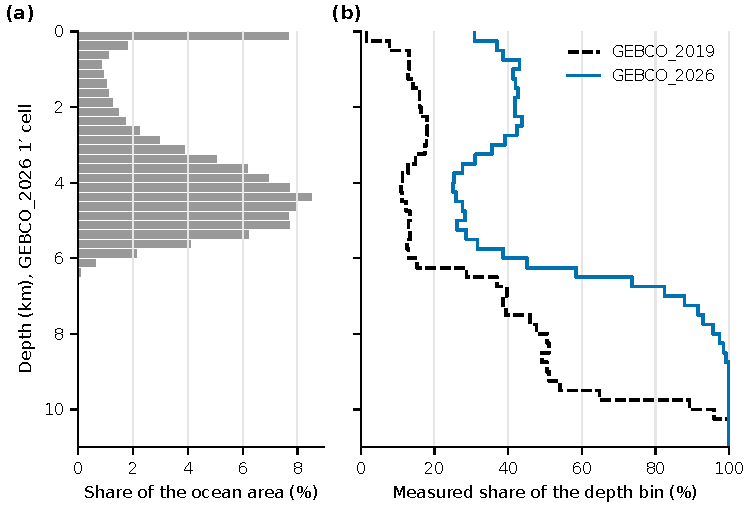
\includegraphics[width=0.8\textwidth]{fig/fig05_depth_2019_2026.pdf}
\caption{(a) Share of the ocean area in each 250\,m depth bin and (b) share of each bin coded as directly measured in GEBCO\_2019 and GEBCO\_2026. Depth is the GEBCO\_2026 1\am\ depth of the cell, used for every release. Data: \texttt{by\_depth\_bin\_by\_release.csv}.}
\label{fig:depth}
\end{figure}

By latitude, the Northern Hemisphere ocean is 38.6\,\% measured in GEBCO\_2026 and the Southern Hemisphere ocean 25.0\,\%.
%% derived from LB 2026: bands with lat_south_deg >= 0: 0.386; lat_north_deg <= 0: 0.250
Outside the bands poleward of 60$^\circ$, the least measured bands are 40--45$^\circ$\,S and 45--50$^\circ$\,S (19.4 and 20.3\,\%).
%% LB 2026: -45..-40 0.194, -50..-45 0.203
By ocean, shares range from 20.5\,\% in the Indian Ocean to 47.4\,\% in the North Atlantic.
%% OC 2026: Indian Ocean 0.2047; North Atlantic Ocean 0.4743
EEZs (139.5 million km$^2$) are 38.0\,\% measured in GEBCO\_2026 and the high seas (221.1 million km$^2$) 26.4\,\%.
%% ZN 2026: eez 139,484,502 km2, 0.37961; high_seas 221,121,369 km2, 0.26416
In GEBCO\_2019 both were 12.5\,\%.
%% ZN 2019: eez 0.12448, high_seas 0.12470
These numbers describe what has been shared with GEBCO; a low share means ``not in the public grid'', not necessarily ``never surveyed''.

\section{Comparison with other estimates}
\label{sec:comparison}

\subsection{\citet{niyazi2025}}

\citet{niyazi2025} counted cells with TID 1 to 17 as mapped (the codes in use are 10 to 17) and 40 to 46 and 70 to 72 as not mapped.
They reprojected the grids to the Mollweide projection (ESRI:54009), resampled the bathymetry onto the TID grid by nearest neighbour, computed areas from pixel counts (planar areas in that projection), took the coastline as the zero-depth line of GEBCO\_2024, and used Global Oceans and Seas version 1 for the ocean basins and the Marine Regions EEZ (version 12) and High Seas data sets, assigning each EEZ to its first-level sovereign.
This dataset uses the same TID codes and the same region data sets, but a different ocean mask, exact spherical areas of the native cells, and the GEBCO\_2026 1\am\ depth for every release.
Their basins are the ten Global Oceans and Seas polygons, which are also the polygons of \texttt{by\_ocean\_by\_release.csv}.
Their per-release global values are in a supplementary table that could not be retrieved from the publisher's page on 16 November 2026, so only the values stated in their text are compared: the global share for 2019 and 2024, and the 2024 (and where given 2019) shares by basin, depth zone and EEZ (Table~\ref{tab:niyazi}).
%% Niyazi et al. (2025) full text read 2026-11-16 (frontiersin.org, Methods and Results); supplementary Table1.docx not downloadable

\begin{table}[t]
\caption{Measured share (\%) in \citet{niyazi2025} and in this dataset for the values stated in their text. Depth zones of this dataset are sums of 250\,m bins of the GEBCO\_2026 1\am\ depth. Sources: \texttt{global\_by\_release.csv}, \texttt{by\_ocean\_by\_release.csv}, \texttt{by\_depth\_bin\_by\_release.csv}, \texttt{by\_zone\_by\_release.csv}.}
\label{tab:niyazi}
\small
\begin{tabular}{lrrrr}
\tophline
 & \multicolumn{2}{c}{2019} & \multicolumn{2}{c}{2024} \\
Group & Niyazi & This & Niyazi & This \\
\middlehline
Global & 12.4 & 12.43 & 28.5 & 28.54 \\
North Atlantic Ocean & & & 44.5 & 44.47 \\
North Pacific Ocean & & & 37.2 & 37.21 \\
South Pacific Ocean & & & 23.4 & 23.43 \\
South Atlantic Ocean & & & 28.1 & 26.83 \\
Indian Ocean & & & 17.5 & 17.51 \\
Depth 1000--3000\,m & 16.8 & 16.71 & 39.2 & 39.03 \\
Depth 3000--6000\,m & 12.7 & 12.75 & 26.2 & 26.22 \\
Depth $>$\,6000\,m & 23.71 & 22.95 & 55.56 & 53.99 \\
EEZ & 13.1 & 12.45 & 33.2 & 35.00 \\
\bottomhline
\end{tabular}
%% G 2019 0.124271, 2024 0.285397; OC 2024: North Atlantic 0.4447, North Pacific 0.3721, South Pacific 0.2343, South Atlantic 0.2683, Indian 0.1751
%% derived from DB (sum of 250 m bins): 1000-3000 m 2019 0.1671, 2024 0.3903; 3000-6000 m 0.1275, 0.2622; >6000 m 0.2295, 0.5399
%% ZN eez 2019 0.12448, 2024 0.35001
%% Niyazi et al. 2025: Results (global, basins, depth zones, EEZ: "13.1% in 2019, and 33.2% in 2024")
\end{table}

The global shares agree to the precision given there.
Four of the five basin shares for 2024 agree to within 0.05 percentage points; the South Atlantic differs by 1.3 points.
The shares at 1000--3000\,m and 3000--6000\,m agree to within 0.2 points in both years.
The shares deeper than 6000\,m differ by 0.8 (2019) and 1.6 points (2024), and the EEZ shares by 0.7 and 1.8 points.
The two analyses differ in the ocean mask, the depth grid, the treatment of EEZ overlaps and coastlines, and the area computation; the comparison does not separate these effects.

\subsection{Official Seabed 2030 figures}

The measured share of the record is 2.6 percentage points below the official figure in 2019 and 0.8 points below in 2020.
From 2021 it is 1.3 to 2.4 points above (Table~\ref{tab:global}, Fig.~\ref{fig:share}).
%% G: 100*measured_share - 100*official: 2019 -2.57, 2020 -0.76, 2021..2026 +1.31 .. +2.44
For 2026, the record has 111.4 million km$^2$ coded as measured, and the announcement gives ``approximately 104 million square kilometres of mapped seabed'' \citep{news2026}.
%% G 2026 measured_area_km2 111,438,640; announcement quote checked 2026-11-15 (docs/paper/references.bib news2026)

The official calculation is not published, so the difference between the two figures cannot be decomposed with this dataset.

\section{Known issues and limitations}
\label{sec:limits}

\begin{itemize}
\item \textit{Definition.} ``Measured'' is GEBCO's own source classification. The dataset does not test whether a cell coded as measured has an accurate depth, or whether one sounding represents a whole cell. The share is a count of cells holding data, not of swath coverage.
\item \textit{Codes 44 and 70 can hold soundings.} GEBCO defines TID 44 as depths ``from multiple sources including measured and derived data'' in a gridded data set guided by satellite gravity, and TID 70 as a pre-generated grid ``based on mixed source data types, e.g. single beam, multibeam, interpolation etc.'' \citep{gebcodoc2026}. Cells with these codes can therefore contain measurements but are counted as not measured, so the 10--17 share is a lower bound on the area holding data. In GEBCO\_2026, codes 44 and 70 cover 3.05\,\% of the mask (1.41 and 1.64\,\%; 8.86\,\% in GEBCO\_2019), and 32.6\,\% of the area re-coded away over all transitions went to them.
%% data/raw/gebco_2026/GEBCO_Grid_docmentation.pdf (pdftotext), TID table; TC 2026 tid 44 0.014129, tid 70 0.016394; 2019 0.030114 + 0.058503; derived from RD: (44 + 70) / total = 0.3256
\item \textit{Cell size.} The east--west width of a 15\as\ cell falls from 463\,m at the equator to 80\,m at 80$^\circ$. Users who need a share on cells of constant width or of another size should use \texttt{cellsize\_sensitivity\_2026.csv} or aggregate the bitmask themselves (Sect.~\ref{sec:cellsize}). The cell-size variants exist for GEBCO\_2026 only.
\item \textit{Re-coding is not data loss.} TID codes change between releases for reasons other than new surveys, for example re-gridding or a source re-classified as a pre-generated grid. ``Re-coded away'' is a property of the GEBCO coding.
\item \textit{First measured is not the survey year.} A release can add surveys collected many years earlier.
\item \textit{Fixed ocean mask.} Using the GEBCO\_2026 mask for every release ignores changes of coastline and ice shelves; each release's own mask changes the share by at most 0.016 percentage points. Water under floating ice shelves is excluded. Areas below sea level that are not connected to the world ocean (931\,885\,km$^2$, mostly the Caspian Sea and the lowland around it) are included in the global figures; they are flagged per cell, and \texttt{global\_by\_release.csv} gives the shares without them (Sect.~\ref{sec:inland}). The flag depends on the grid: an inlet whose link to the sea is narrower than one 15\as\ cell is flagged.
%% G max own-mask difference 0.000158; G inland_below_sea_level_area_km2
\item \textit{Input versions.} The GEBCO\_2023 TID grid was re-issued without a new DOI or netCDF metadata (Sect.~\ref{sec:inputs}). Other releases may change in the same way. The inputs are identified by their SHA-256 checksums in \texttt{inputs.sha256}; the dataset describes the TID files as distributed by CEDA in November 2026 and the elevation as served by the Source Cooperative copy (last modified 7 May 2026), which was compared with the official grid at six sites only.
\item \textit{Shared is not surveyed.} National and commercial surveys that are not contributed to GEBCO count as not measured.
\item \textit{Region boundaries.} The Marine Regions polygons were taken from generalised GeoServer output (Sect.~\ref{sec:inputs}) and rasterised by cell centre on a 1\am\ grid, so boundaries are accurate to about one 1\am\ cell (about 1.9\,km). Small EEZs therefore carry errors of a few percent. For 2026, the EEZ share is 37.961\,\% in this dataset and 37.951\,\% in the regional pipeline, which stores 1\am\ measured fractions in steps of 1/254.
%% DR "Tables" last paragraph: 37.961 vs 37.951 %
\item \textit{Area model.} Areas are computed on the authalic sphere with geodetic latitudes; against WGS84 ellipsoidal areas the ocean area of a 5$^\circ$ band is off by $-0.89$ to $+0.45$\,\% and the global share by at most 0.011 percentage points (Sect.~\ref{sec:methods}).
\item \textit{No uncertainty on the shares.} The percentages are exact sums under a stated definition. Their uncertainty is one of definition (cell size, grouping of codes), not of sampling.
\item \textit{Metadata.} The ACDD attributes \texttt{creator\_email} and \texttt{publisher\_*} are not set in version 1.0.0 of the file; the repository record carries this information.
\end{itemize}

\conclusions

The dataset records, for every 15\as\ cell of the global grid, in which of the eight GEBCO releases 2019 to 2026 the cell is coded as directly measured.
It reproduces the measured share of each release from public files, from 12.4\,\% in 2019 to 30.8\,\% in 2026; the global shares for 2019 and 2024 equal those of \citet{niyazi2025} to the precision given there, and their 2024 shares by basin, depth zone and EEZ differ from those of this dataset by 0.01 to 1.8 percentage points (Table~\ref{tab:niyazi}).
%% G 0.12427, 0.30810
The record shows that the TID coding is not cumulative: each transition moves 0.8 to 4.6 million km$^2$ out of the measured codes, and 33.0\,\% of the seafloor has been coded as measured in at least one release.
%% G recoded_away_vs_previous_km2 range; ever_measured_share_fraction 2026
It also shows that a share based on one sounding per cell depends on the cell size, from 30.8\,\% on native cells to 37.7\,\% on blocks of about 1.85\,km.
%% CS native 0.30810, ew4_any 0.37654
Two practical points follow for users.
A study that uses one release's TID grid as a mask of measured cells should name the release, because the mask can change by millions of square kilometres between releases without any new survey.
And a coverage figure should be reported together with the cell size and counting rule used.
The dataset can be extended with each new GEBCO release by adding one bit to the mask and one row per group to each table.

\codedataavailability{%
The dataset described here, version 1.0.0 (the netCDF file, the ten tables, the README with the data dictionary, the two checksum files \texttt{inputs.sha256} and \texttt{checksums.sha256}, and the two reports \texttt{verify.log} and \texttt{compliance\_checker.txt}), is available from Zenodo at \url{https://doi.org/\datasetdoi} \citep{ismoilov2026data} under the Creative Commons Attribution 4.0 International licence (CC BY 4.0).
It is derived from the GEBCO\_2019 to GEBCO\_2026 grids (GEBCO Compilation Group; DOIs in the reference list), which are in the public domain under the GEBCO terms of use, with attribution required (CEDA lists the Open Government Licence v3 for the 2025 and 2026 releases), and from Marine Regions data sets (Flanders Marine Institute, CC BY 4.0).
Suggested attribution: ``Contains data from the GEBCO\_2019--GEBCO\_2026 Grids (GEBCO Compilation Group) and Marine Regions (Flanders Marine Institute, CC BY 4.0).''
The inputs are not redistributed. The TID grids can be downloaded from the cited DOIs (CEDA), the GEBCO\_2026 elevation was read from the Source Cooperative copy \citep{aad2026gebcocog}, the Marine Regions layers from the Marine Regions GeoServer (Sect.~\ref{sec:inputs}), and \texttt{inputs.sha256} identifies the exact files used.
The code that builds, tabulates and verifies the dataset (\texttt{pipeline/history.py}, \texttt{pipeline/build\_dataset.py}, \texttt{pipeline/sensitivity\_cellsize.py}) and the figure script of this paper (\texttt{docs/essd/figures.py}) are released under the MIT licence at \url{https://github.com/ismoilovdevml/seafloor-atlas} and archived on Zenodo at \url{https://doi.org/\codedoi} \citep{ismoilov2026code}; the concept DOI for all versions of the code is 10.5281/zenodo.24228190.
The commands \texttt{inputs}, \texttt{connectivity}, \texttt{build}, \texttt{tables}, \texttt{verify} and \texttt{checksums} of \texttt{pipeline/build\_dataset.py} and the compliance checker regenerate every file of the dataset from the inputs.}

\authorcontribution{%
Otabek Ismoilov: Conceptualization, Supervision, Project administration, Validation, Writing -- review \& editing.
The use of an AI assistant is described in Sect.~\ref{sec:ai}.}

\competinginterests{The author declares that they have no conflict of interest.}

\begin{acknowledgements}
The author thanks the GEBCO Compilation Group and the Seabed 2030 regional and global data centres for releasing the grids and their Type Identifier grids openly, CEDA for hosting the archives, the Flanders Marine Institute for the Marine Regions data, and the Australian Antarctic Division for the cloud-optimised copy of the GEBCO grid. Code, analyses, figures and the first manuscript text were produced with the AI assistant Claude (Anthropic) through Claude Code, model claude-opus-5-5, under the author's direction; see Sect.~\ref{sec:ai}. This work received no specific funding.
\end{acknowledgements}

\bibliographystyle{copernicus}
\bibliography{references}

\end{document}
